\documentclass[12pt]{article}
\usepackage[a4paper, left=3.17cm, right=3.17cm, top=2.54cm, bottom=2.54cm]{geometry}
\usepackage[T1]{fontenc}
\usepackage{mathptmx}
\usepackage{amsmath}
\usepackage{ctex}
\usepackage{amsfonts}
\usepackage{chemformula}
\usepackage{cite}
\usepackage{float}
\usepackage{setspace}
\usepackage[colorlinks, linkcolor=black, anchorcolor=black, citecolor=black]{hyperref}
\usepackage{graphicx}
\setlength{\parskip}{0.5em}
\doublespacing
\title{四波分WDM光纤传输系统}
\author{202011010101孙陶庵,202011010103葛家乐,202011010110张钧赫}
\begin{document}

    %——————————————————————————————————设置公式编号———————————————————————————————————————%
    \numberwithin{equation}{subsection}
    \renewcommand\theequation{\thesubsection.\arabic{equation}}
    %%%%%%%%%%%%%%%%%%%%%%%%%%%%%%%%%%%%%%%%%%%%%%%%%%%%%%%%%%%%%%%%%%%%%%%%%%%%%%%%%%%%%%
    \newtheorem{mythm}{定理}[section]  %定义一个定理环境
    %\maketitle  

    \begin{titlepage}
      \newcommand{\HRule}{\rule{\linewidth}{0.5mm}}
      
\includegraphics[width=12.5cm]{sc_logo.jpg}\\[0cm] 
      \center 
      \quad\\[1cm]
      \textsl{\Large 湖南大学 }\\[0.5cm] 
      \textsl{\large 物理与微电子科学学院}\\[-0.5cm] 
      \makeatletter
      \HRule \\[0.4cm]
      { \huge \bfseries \@title}\\[0.4cm] 
      \HRule \\[1.5cm]
      \begin{minipage}{0.4\textwidth}
        \begin{flushleft} \large
          \emph{Author:}\\
          \vspace{0pt} % 将文字部分向上移动
          \@author 
        \end{flushleft}
      \end{minipage}
      ~
      \begin{minipage}{0.4\textwidth}
        \begin{flushright} \large
          \emph{Supervisor:} \\
          \vspace{0pt} % 将文字部分向上移动
          \textup{黄维清}
        \end{flushright}
      \end{minipage}\\[3cm]
      \makeatother
      {\large 物理2001班}\\[0.5cm]
      {\large \emph{光电子学基础实践课}}\\[0.5cm]
      {\large \today}\\[2cm] 
      \vfill 
    \end{titlepage}
\thispagestyle{empty}
\clearpage     %另起一页  
\pagenumbering{arabic}
\tableofcontents        %输出目录
\clearpage     %另起一页 

\section{摘要}
本报告旨在设计一个$4\times 5 Gbit/s$的长距离光纤传输系统,并利用OptiSystem进行仿真验证。设计过程中采用了波分复用技术,
通过多通道传输实现高速数据传输。传输距离设定为100 km,选择常规光纤作为传输介质,光纤损耗系数为0.25 dB/km。
系统中引入了EDFA作为线路放大器,用于补偿传输距离引起的信号衰减。设计的目标是优化系统性能,使系统接收端的输入功率和光信号噪声比
(OSNR)达到最佳水平。通过仿真试验和设计优化,能够实现高速、长距离数据传输的可靠性和稳定性。最终的设计方案将提供设计图和仿真结果,
以验证系统的性能和有效性。该光纤传输系统的成功设计和实施将对满足现代高容量数据传输的需求具有重要意义。

关键字:光纤传输系统、波分复用技术、2.5 Gbit/s、长距离传输、OptiSystem仿真、多通道传输
\clearpage     %另起一页 
\section{设计背景}
随着信息技术的迅速发展,对高速、高容量数据传输的需求不断增长。在长距离传输场景中,光纤传输系统成为了一种理想的解决方案,
具有较低的信号衰减、较高的带宽和抗干扰能力。

本次设计任务是设计一个$4\times 5 Gbit/s$的长距离光纤传输系统,并利用OptiSystem仿真验证。设计的目标是实现高速、长距离数据传输,
并通过优化设计方案达到系统接收端的最佳输入功率和光信号噪声比(OSNR)。

在设计过程中,考虑到以下背景和需求:
\\
1.传输速率和容量要求:随着数据量的不断增长,传输速率和容量成为设计的重要考虑因素。
为了满足高速数据传输的需求,传输速率被设定为 5 Gbit/s。通过采用波分复用技术,利用多通道传输的方式,可以有效提高系统的容量和传输速率。
\\
2.长距离传输需求:在一些应用场景中,需要在远距离范围内进行数据传输,如跨越城市或跨越国家。
因此,传输距离被设定为100 km。在长距离传输中,光纤的损耗和衰减会对信号质量和功率产生不利影响,因此需要采取相应的措施来补偿信号损耗。
\\
3.	光纤材料和损耗系数:为了满足设计要求,常规光纤被选择为传输介质。常规光纤具有较低的损耗系数,为0.25 dB/km,
可以有效减少光信号在传输过程中的衰减和损耗。
\\
4.	线路放大器:为了补偿传输距离引起的信号衰减,设计中引入了EDFA(掺铒光纤放大器)作为线路放大器。
EDFA具有较大的增益范围和较低的噪声指数,可以增强光信号的功率,并提高系统的传输性能。
\\
综上所述,本次设计的背景是满足高速、长距离数据传输的需求。通过采用波分复用技术、合适的光纤材料和线路放大器配置,
旨在设计一个高效可靠的光纤传输系统,以实现优化的数据传输性能
\subsection{系统原理}
波分复用器的系统原理基于光的波长多路复用技术。该技术利用光的波长作为信息的载体,
将不同波长的光信号同时传输在同一根光纤中,实现多信道的并行传输。

具体来说,波分复用器通过将多个输入光信号引入不同的通道,
并通过适当的光学元件将它们合并到一个光纤中。在接收端,光信号经过解复用器,通过相应的分路器将不同波长的信号分离出来,
然后经过光电转换器将它们转换为电信号进行处理和解码。

波分复用器的核心元件是光栅。光栅是一种具有周期性折射率变化的光学元件,通过其特殊的结构和折射率分布,
可以实现波长选择和光信号的分光。光栅通常采用光纤光栅或光栅片的形式,其结构中包含周期性的折射率变化区域。
当入射光信号经过光栅时,不同波长的光信号会受到不同的衍射效应,从而被分离到不同的输出通道中。

除了光栅,波分复用器还包括耦合器、滤波器和光纤等组件。耦合器用于将不同波长的光信号引入波分复用器的不同通道,
滤波器用于选择特定波长的光信号进行复用,光纤用于将复用后的信号传输到目标位置。
\begin{figure}[htbp]
	\centering
	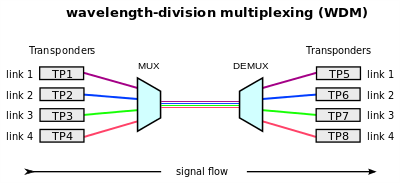
\includegraphics[width=8cm]{figure1.png}
	\caption{波分复用器示意图}
\end{figure}
\clearpage
\section{设计目的}
本次设计的主要目的是设计一个$4\times 5 Gbit/s$的长距离光纤传输系统,并利用OptiSystem进行仿真验证。以下是设计目的的具体说明:\\
1.	高速数据传输:设计的系统旨在实现高速数据传输,每个通道的传输速率为5 Gbit/s。通过合理的波分复用技术和多通道传输配置,
系统可以同时传输多个通道的数据,满足大容量数据传输的需求。
\\
2.	长距离传输:设计考虑了长距离传输的需求,传输距离为100 km。在传输过程中,光信号会受到光纤损耗和衰减的影响,
设计的目的是通过优化设计方案,确保在长距离传输中保持信号的质量和功率。
\\
3.	优化系统性能:通过仿真验证和优化设计方案,旨在达到系统接收端的最佳输入功率和光信号噪声比(OSNR)。
优化系统性能可以提高数据传输的可靠性和稳定性,确保接收端能够准确、高效地解码和处理光信号。
\\
4.	考虑损耗要求:设计过程中仅考虑损耗要求,通过选择合适的光纤材料和线路放大器配置,以最小化信号的衰减和损耗。
优化损耗可以减少信号传输过程中的噪声和失真,提高系统的传输性能和可靠性。
\\
通过实现以上设计目的,可以构建一个高速、长距离的光纤传输系统,并通过仿真验证和优化设计方案,确保系统的性能达到预期要求,满足现代高速数据传输的需求。
\section{问题的提出与分析}
在我们的设计过程中,我们主要关注了以下几个问题,并通过详细分析和解决方案来确保设计的可靠性和性能优化。

首先,我们面临的问题是如何在实验中仿真输入随机的信号以模拟实际信号传输。在光纤传输系统中,我们需要考虑不同信号的传输特性和噪声情况。
为了解决这个问题,我们选择利用OptiSystem提供的随机信号生成器来生成具有随机性质的信号,并将其用于仿真环境中进行传输性能评估。
这样,我们可以模拟真实信号的统计特性和传输效果,为系统设计和性能分析提供准确的数据基础。

其次,我们需要解决传输过程中可能出现的损失和误差问题。光纤传输系统存在信号衰减、色散、干扰等因素,可能导致信号失真和传输质量下降。
为了应对这些问题,我们在设计中引入了色散补偿器和光放大器等器件。色散补偿器可以校正光信号在传输过程中的色散效应,
而光放大器则可以增强信号强度以克服传输距离引起的衰减。此外,我们还采取了滤波和干扰抑制等技术来减少传输过程中的干扰。通过这些措施,
我们能够最大程度地降低信号损失和误差,提高传输质量和可靠性。

最后,我们关注的是对传输结果的测量和比对。在复分复用的光纤传输系统中,我们需要对信号进行解复用并测量关键性能指标,如误码率(BER) 
\cite{enwiki:1158016020}和Q因子\cite{HICKMAN199025}。为了实现这一目标,我们使用BER分析仪对输出信号进行评估和分析。通过观察和分析眼图、BER曲线以及其他统计特性,
我们能够准确评估传输质量,并根据结果进行系统优化和改进。这些测量和比对结果对于验证设计方案的可行性和性能达标性具有重要意义。

通过解决上述问题并提出相应的解决方案,我们能够确保光纤传输系统设计具有高可靠性和优秀的性能表现。在实际应用中,
我们的设计方案可以为长距离数据传输提供可靠保障,并为未来光纤通信系统的发展提供参考和借鉴。
\begin{figure}[htbp]
	\centering
	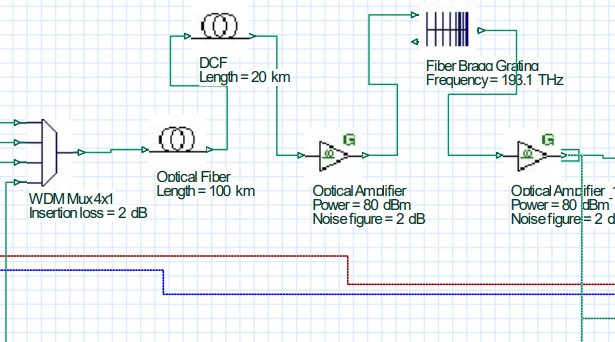
\includegraphics[width=8cm]{figure2.png}
	\caption{引入的色散补偿器和光放大器}
\end{figure}
\clearpage
\section{设计方案}
我们这里的设计方案主要分为三个部分:
\subsection{波分前}
在我们的设计方案中,第一部分是波分前(Wavelength Division Front)的部分。
这部分主要包括四个通道,其中涉及到两个关键组件,即随机信号生成器和MZ调制器。下面将详细说明这两个组件的作用。
\subsubsection*{随机信号生成器}
随机信号生成器是光纤传输系统中的重要组件之一。其主要作用是生成高质量的随机信号,
用于调制光信号。在本设计中,我们采用随机信号生成器来产生用于调制的随机二进制序列。这些随机二进制序列将作为传输数据流的基础,
通过调制将其转换为光信号,以便在光纤传输系统中进行传输。随机信号生成器的输出应具有良好的随机性、平均功率和低误码率,
以确保数据传输的可靠性和性能。
\subsubsection*{MZ调制器}
MZ调制器(Mach-Zehnder Modulator)是光通信系统中常用的调制器之一。它基于Mach-Zehnder干涉原理,
通过调节两个平行的光路之间的干涉效应来实现光信号的调制。在本设计中,我们使用MZ调制器对随机信号进行调制,将其转换为光信号。
调制后的光信号将具有随机信号携带的信息,以便在光纤传输中进行传输。MZ调制器具有高速调制能力、低插入损耗和良好的调制深度,
能够保持信号的完整性和质量。
\subsubsection*{总的}
通过将随机信号生成器和MZ调制器结合起来,波分前部分将实现每个通道的数据调制和信号转换。随机信号生成器将产生高质量的随机二进制序列,
MZ调制器将利用这些序列对光信号进行调制,使其具备传输所需的信息和特性。这样,我们就能够准备好传输到下一部分的调制光信号,
为光纤传输系统的正常运行打下坚实的基础。

\subsection{中间部分}
在我们的设计方案中,第二部分是中间部分,也称为光纤传输部分。这部分起着连接和传输调制光信号的关键作用。
下面将详细说明中间部分的各个组件的作用以及解决的误差问题。
\subsubsection*{光纤传输部分}
光纤是光通信系统中传输光信号的基本媒介。在中间部分,我们使用常规光纤来承载和传输经过调制的光信号。
光纤的主要作用是提供可靠的传输通道,将调制光信号从发送端传输到接收端。在设计中,我们需要考虑光纤的损耗系数和传输距离,
以确保信号在传输过程中能够保持足够的强度和质量。
\subsubsection*{误差修正和校正}
在光纤传输过程中,由于光纤本身的特性以及传输过程中的各种因素,会导致信号受到一定的失真和干扰,
从而产生误差。为了解决这些误差问题,我们需要引入误差修正和校正技术。这可以包括使用前向纠错码(Forward Error Correction, FEC)
来纠正和校正传输中的误码,以及采用均衡器和增益控制器等技术来调整信号的传输特性,使其尽可能地接近原始信号。
\subsubsection*{中端输出显示设备}
中端输出显示设备是接收和显示传输系统输出内容的设备。在设计中,我们需要考虑这些设备的性能和要求,
以确保传输系统输出的信号能够被准确、清晰地显示和解读。这些设备可以包括光接收机、光解调器、解码器和显示器等,
主要作用是接收和解析传输过来的光信号,并将其转换为可视化的输出内容。
\subsubsection*{后面}
通过中间部分的组件和功能,我们能够克服光纤传输过程中的误差和失真问题,并将调制光信号准确地传输到输出显示设备。
这样,我们可以确保传输系统输出的信号具备高质量、可靠性和可解读性,满足用户的需求和期望。
\subsection{后端输出}
在我们的设计方案中,第三部分是后端输出部分,也称为末端。这部分主要涉及信号接收和眼图显示。下
面将详细说明后端输出部分的功能和作用。
\subsubsection*{信号接收}
在后端输出部分,我们使用光接收机来接收光纤传输部分传输的光信号。光接收机的主要作用是将光信号转换为电信号,
以便进一步处理和解读。它通过接收和解调光信号,并将其转换为电压或电流信号,以供后续的信号处理和分析。
\subsubsection*{眼图显示}
眼图是一种用于分析和评估数字信号质量的重要工具。在后端输出部分,我们使用眼图显示设备来显示和分析接收到的信号的眼图。
眼图显示设备通过对接收信号进行采样和重建,绘制出眼图,即信号在时间域中的打开和闭合眼形状。通过观察眼图的特征,
我们可以评估信号的时钟同步性、噪声水平、失真程度等,并进行系统性能的分析和优化。
\\
通过后端输出部分的信号接收和眼图显示功能,我们能够实时监测和评估传输系统的性能。通过分析眼图的特征,
我们可以了解信号在传输过程中是否受到了失真、噪声或其他干扰的影响,进而调整和优化系统的参数和配置,以提高传输质量和可靠性。
\\

我们的设计方案分为三个部分:波分前、中间部分和后端输出。在波分前部分,我们通过随机信号生成器和MZ调制器生成多个波长的光信号。
中间部分包括光纤连接和EDFA放大器,确保信号在光纤中传输质量和强度的保持。后端输出部分涉及信号接收和眼图显示,用于实时监测传输系统性能。
通过这些部分的协同工作,我们能够构建出一个可靠、高效的光纤传输系统,满足高速数据传输和波分复用的需求。
\begin{figure}[htbp]
	\centering
	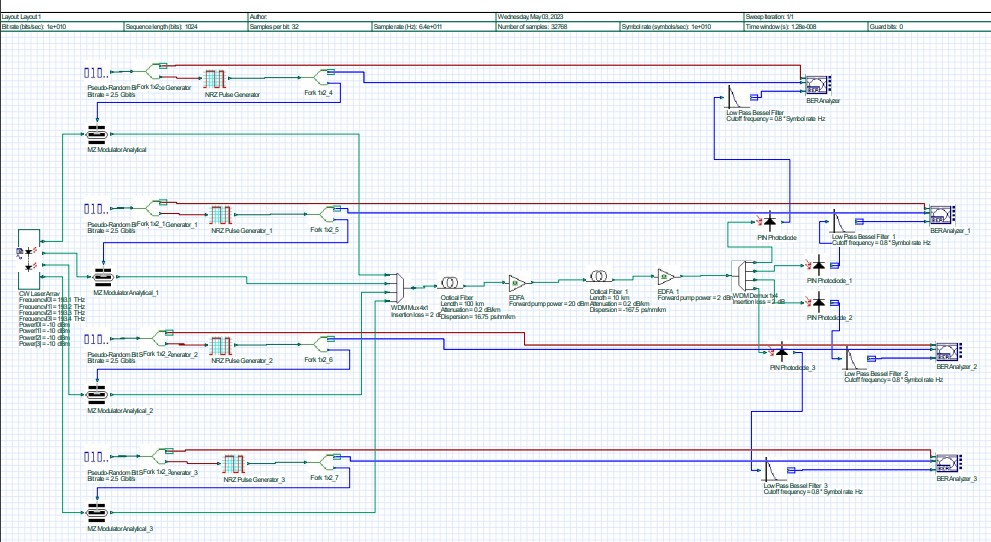
\includegraphics[width=8cm]{figure3.png}
\end{figure}
对于该内容的初始参数设置,如下:
\begin{figure}[H]
  \begin{minipage}[t]{0.5\linewidth}
      \centering
      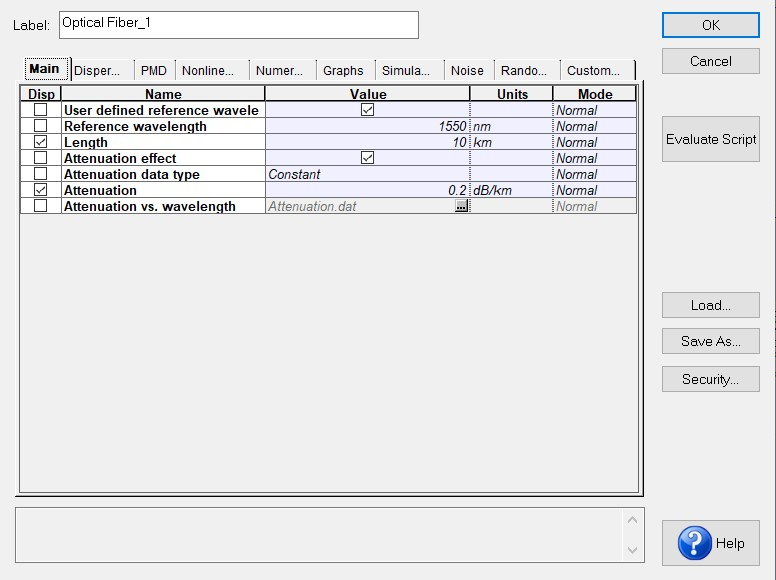
\includegraphics[scale=0.4]{figure4.png}
      \caption{}
      \label{fig:side:a}
    \end{minipage}%
    \begin{minipage}[t]{0.5\linewidth}
      \centering
      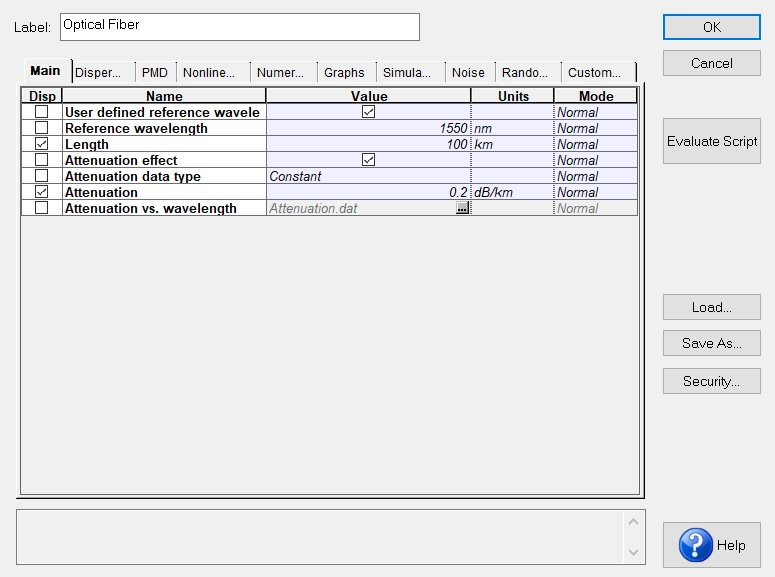
\includegraphics[scale=0.4]{figure5.png}
      \caption{}
      \label{fig:side:b}
    \end{minipage}
\end{figure}

\clearpage
\section{设计内容}

原本的系统存在一些问题,如信号干扰和色散效应,这些问题可能会对系统的性能和输出结果产生不利影响。信号干扰可能导致信号质量下降,
引入噪声和失真,从而使接收端的信号解析能力降低。而色散效应会导致不同频率的光信号在传输过程中相位偏移和传输速度差异,
进而造成信号失真和时域畸变。

为了克服这些问题,我们需要采取一系列措施来提升系统性能和确保准确的输出结果。首先,我们可以引入适当的信号处理技术,
如均衡和前向纠错码等,以降低信号干扰对传输质量的影响。这些技术可以在接收端对信号进行重构和修复,提高信号的可靠性和准确性。

其次,针对色散效应,我们可以采用色散补偿技术,如色散补偿器和色散补偿光纤等。这些补偿器可以根据不同波长的信号特性进行精确调节,
以消除色散引起的相位偏移和传输速度差异,从而保持信号的完整性和稳定性。

此外,我们还可以优化光纤传输路径和组件布局,采用抗干扰设计和合适的信号隔离措施,以降低外界干扰对系统的影响。
通过合理的系统设计和配置,我们可以最大程度地减少信号干扰和色散效应对系统性能的影响,确保输出结果的准确性和稳定性。

因此,为了解决信号干扰、色散等问题,并保证系统的可靠性和输出结果的准确性,
我们需要综合运用信号处理技术、色散补偿技术以及优化系统设计和布局等方法。通过这些措施的综合应用,我们可以提升系统性能,
克服潜在问题,实现高质量的输出结果。

所以我们参考了这篇文章\cite{BHATTACHARJEE2022168598},旨在解决以上问题:
文章中的设计方案是一个32通道256 Gbps的DWDM(密集波分复用)光学系统。在该系统中,
我们采用了色散补偿器(DCF)和光纤光栅(FBG),这些组件的作用是解决长距离数据传输中的色散问题,以提供卓越的传输质量和性能。

首先,我们使用了色散补偿器(DCF),它是一种用于补偿光纤中色散引起的信号失真的设备。在长距离传输中,
光信号会受到色散效应的影响,导致信号的扩散和形状畸变。通过在系统中引入DCF,它能够精确地补偿不同波长的信号的色散,
使得它们能够以更稳定和准确的方式传输,从而提高传输质量和可靠性。

其次,我们还采用了光纤光栅(FBG)作为另一种色散补偿器。光纤光栅是一种具有周期性折射率调制的光纤结构,
通过其特殊的光学特性可以实现对光信号的频率选择性反射和衍射。在光学系统中,我们将光纤光栅放置在合适的位置,
以调整不同波长光信号的传输速度,以实现色散的补偿。这样可以有效地解决不同波长信号传输速度差异引起的相位偏移和色散问题,
进一步提升传输质量和稳定性。成品如下所示:

\begin{figure}[htbp]
	\centering
	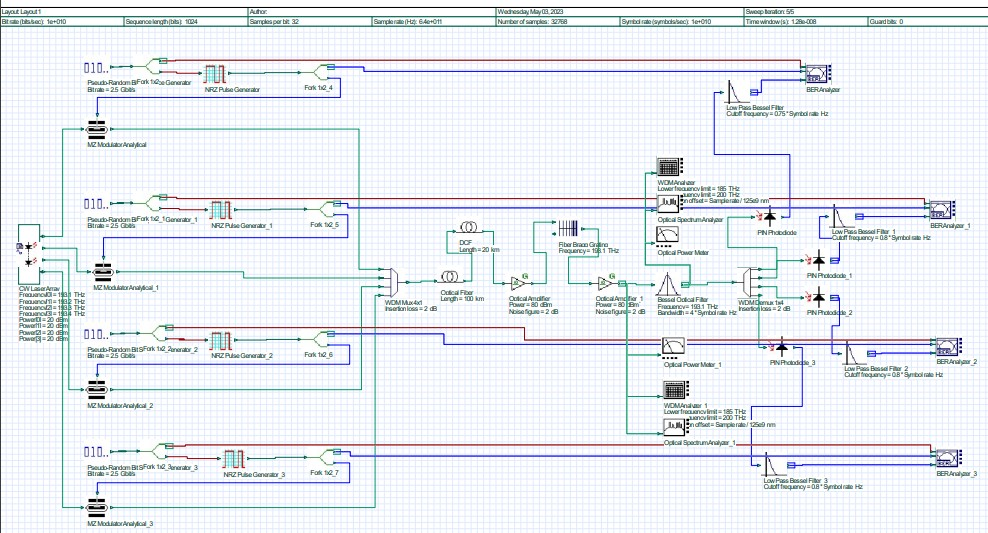
\includegraphics[width=8cm]{figure6.png}
\end{figure}

\begin{figure}[htbp]
	\centering
	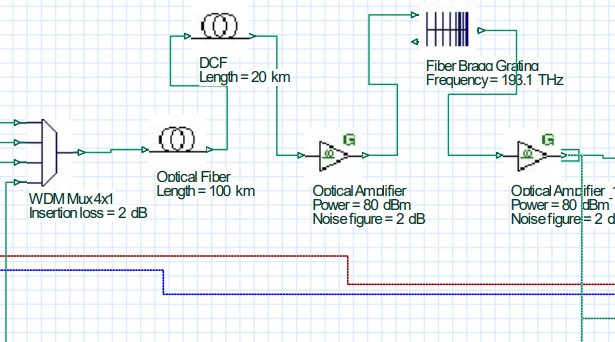
\includegraphics[width=8cm]{figure7.png}
	\caption{改进的部分}
\end{figure}
\clearpage
\section{设计(计算、仿真)结果}

在这个实验中,我们进一步研究了输入源功率对比特损失率的影响。通过增加输入源功率,我们观察到比特损失率呈现出明显的提升现象。
下面的四个图表显示了在输入源功率为0dB时,对应于193.1THz、193.2THz、193.3THz和193.4THz信号的眼图、Q因数和BER数据。
在进行仿真运算时,我们可以发现在不加色散补偿器和光放大器时Q因数的数据:
\begin{figure}[H]
    \begin{minipage}[t]{0.5\linewidth}
        \centering
        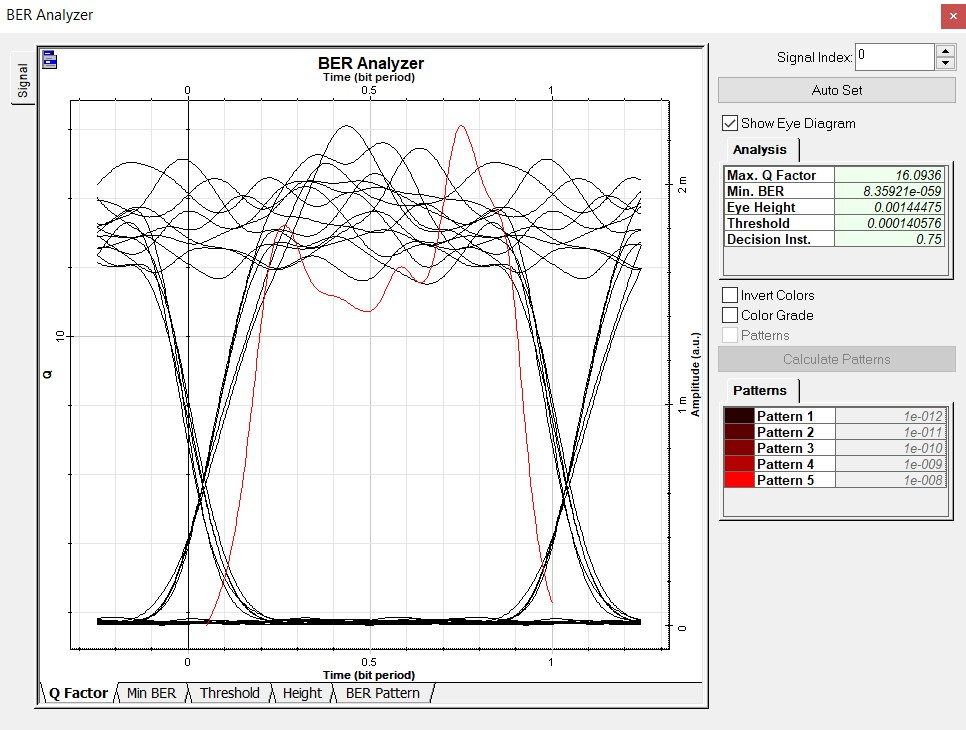
\includegraphics[scale=0.3]{Q-factor (1).jpg}
        \caption{}
        \label{fig:side:a}
      \end{minipage}%
      \begin{minipage}[t]{0.5\linewidth}
        \centering
        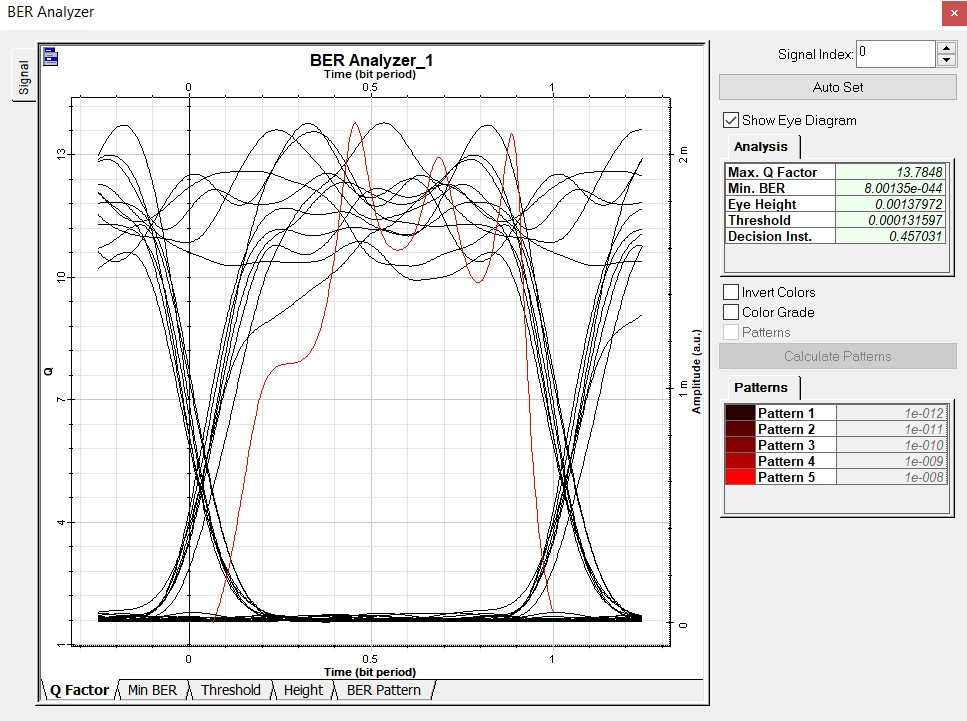
\includegraphics[scale=0.3]{Q-factor (2).jpg}
        \caption{}
        \label{fig:side:b}
      \end{minipage}
	  \begin{minipage}[t]{0.5\linewidth}
        \centering
        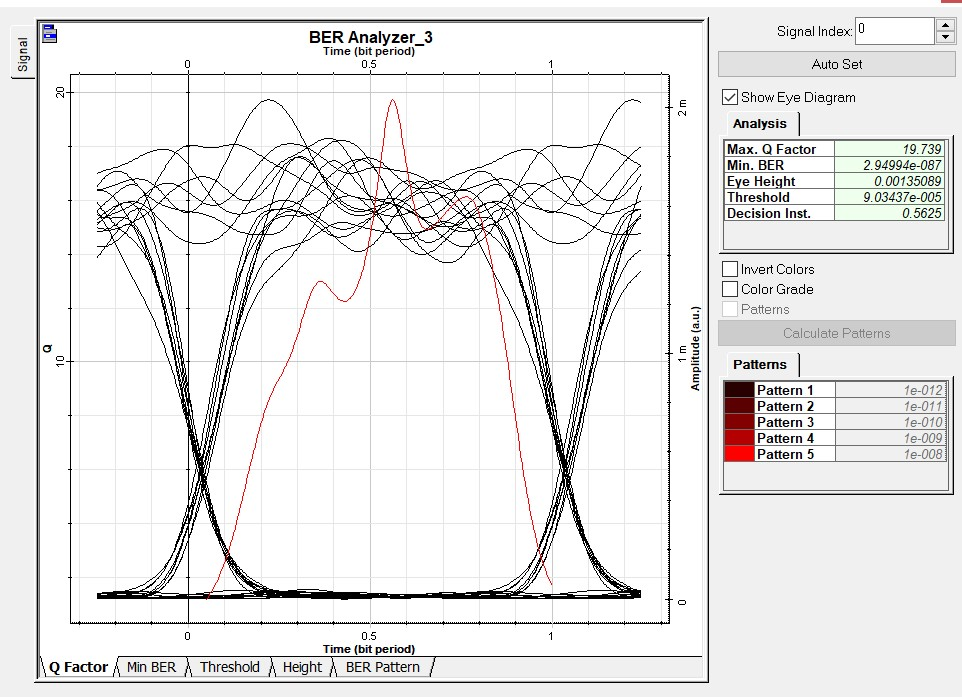
\includegraphics[scale=0.3]{Q-factor (3).jpg}
        \caption{}
        \label{fig:side:a}
      \end{minipage}%
      \begin{minipage}[t]{0.5\linewidth}
        \centering
        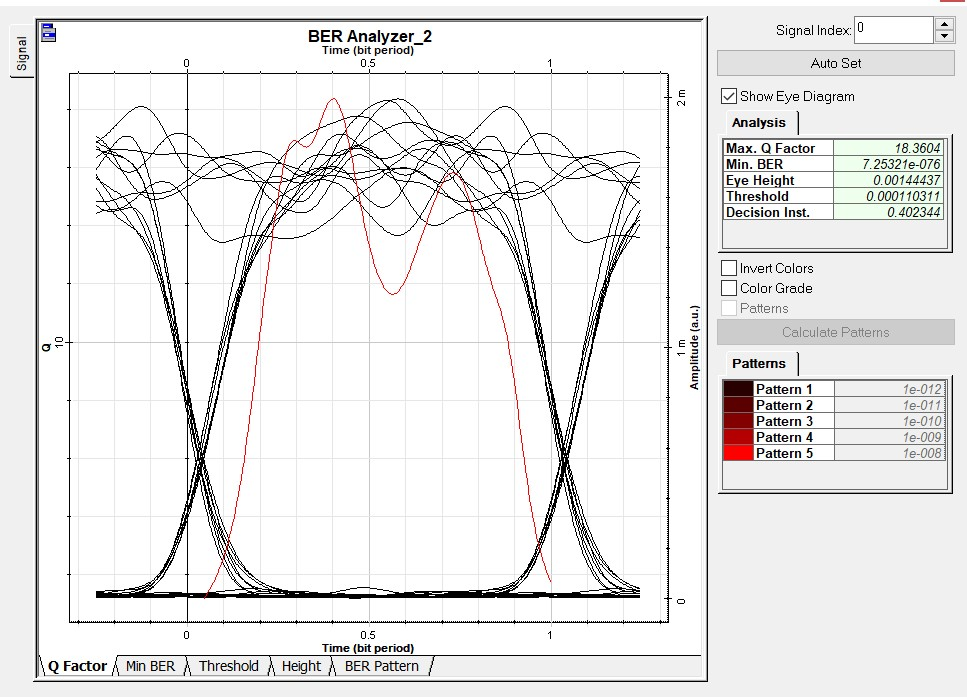
\includegraphics[scale=0.3]{Q-factor (4).jpg}
        \caption{}
        \label{fig:side:b}
      \end{minipage}
\end{figure}

接着是BER:

\begin{figure}[H]
    \begin{minipage}[t]{0.5\linewidth}
        \centering
        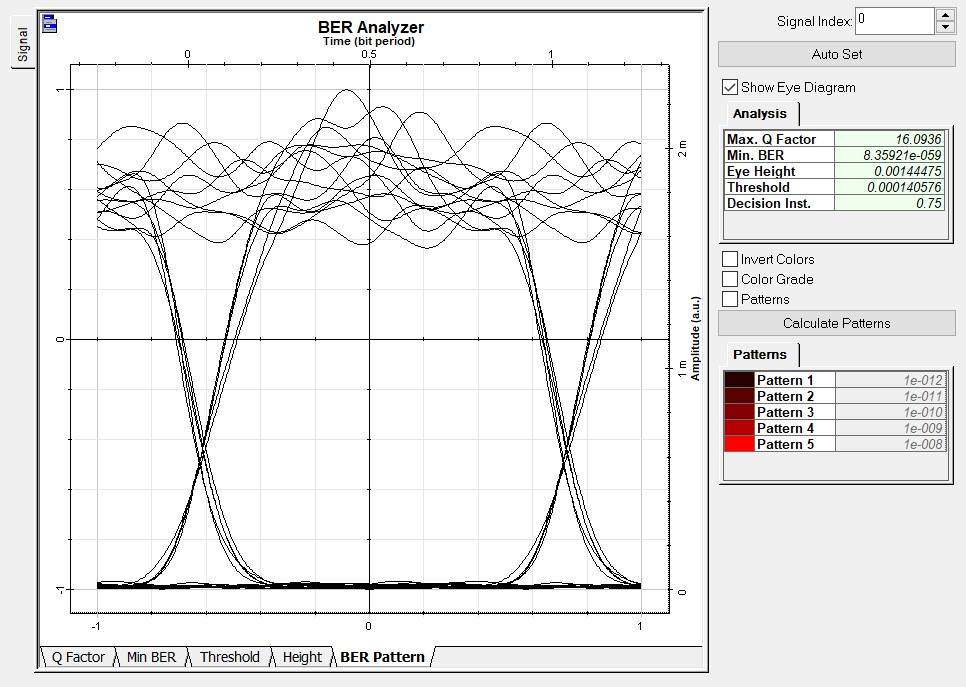
\includegraphics[scale=0.3]{1-BER.jpg}
        \caption{}
        \label{fig:side:a}
      \end{minipage}%
      \begin{minipage}[t]{0.5\linewidth}
        \centering
        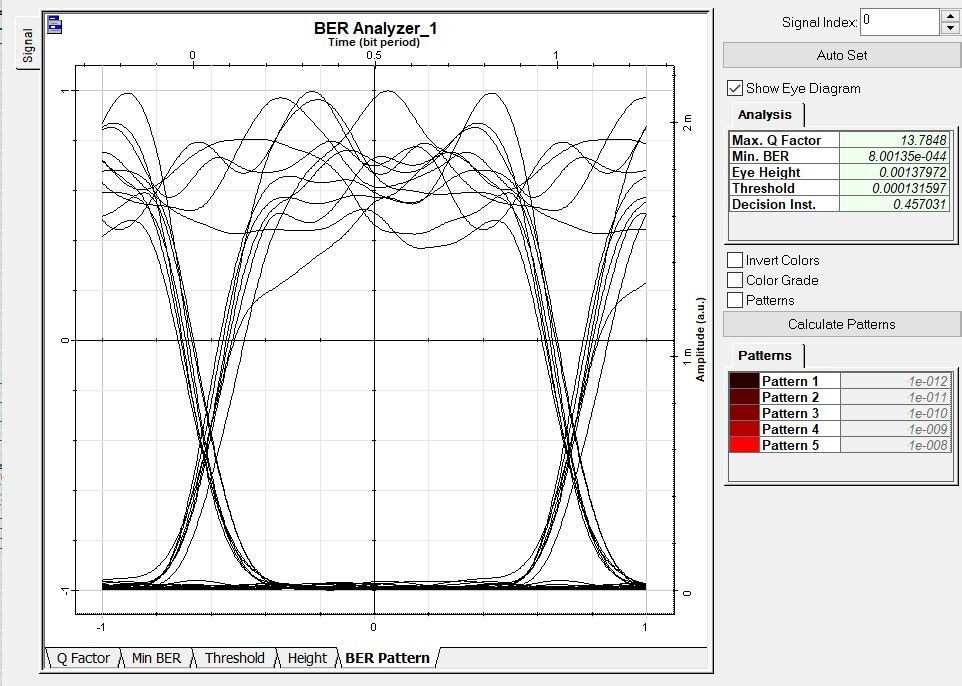
\includegraphics[scale=0.3]{2-BER.jpg}
        \caption{}
        \label{fig:side:b}
      \end{minipage}
	  \begin{minipage}[t]{0.5\linewidth}
        \centering
        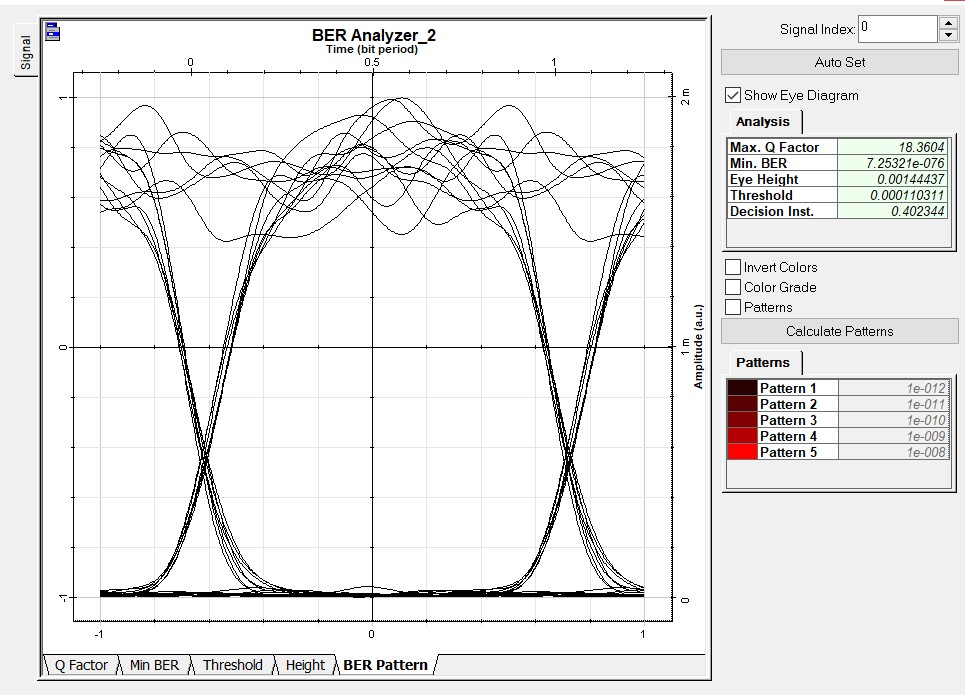
\includegraphics[scale=0.3]{3-BER.jpg}
        \caption{}
        \label{fig:side:a}
      \end{minipage}%
      \begin{minipage}[t]{0.5\linewidth}
        \centering
        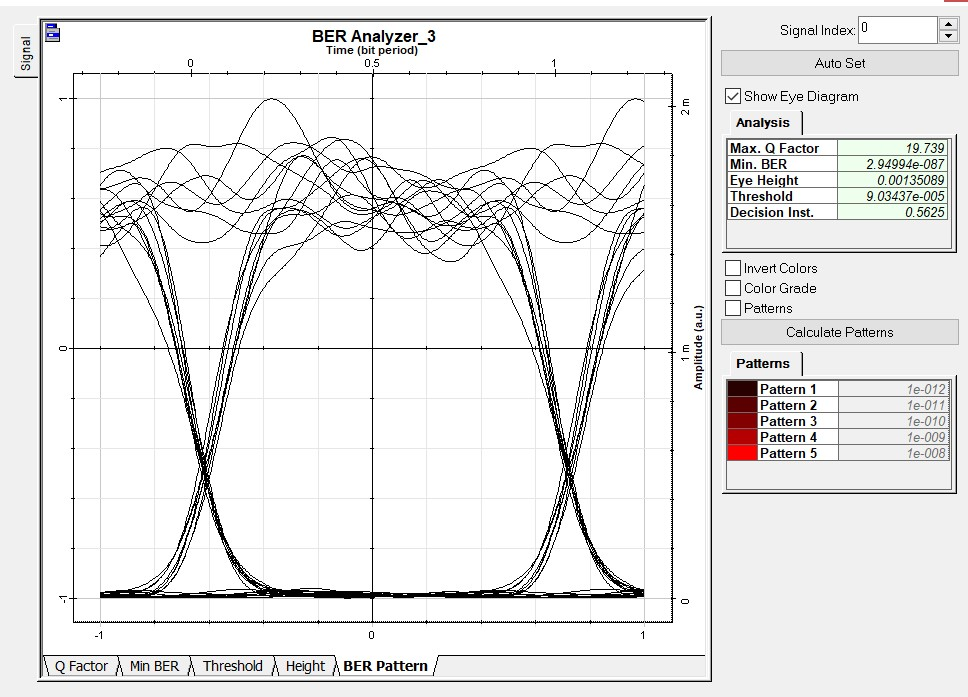
\includegraphics[scale=0.3]{4-BER.jpg}
        \caption{}
        \label{fig:side:b}
      \end{minipage}
\end{figure}

接着与加上了色散和放大器后的进行比对。
我们对该实验进行了数次仿真运算,如下为其中一次运算中sweep2(即当输入源为5dB时)的四个BER分析仪的仿真结果:

\begin{figure}[H]
    \begin{minipage}[t]{0.5\linewidth}
        \centering
        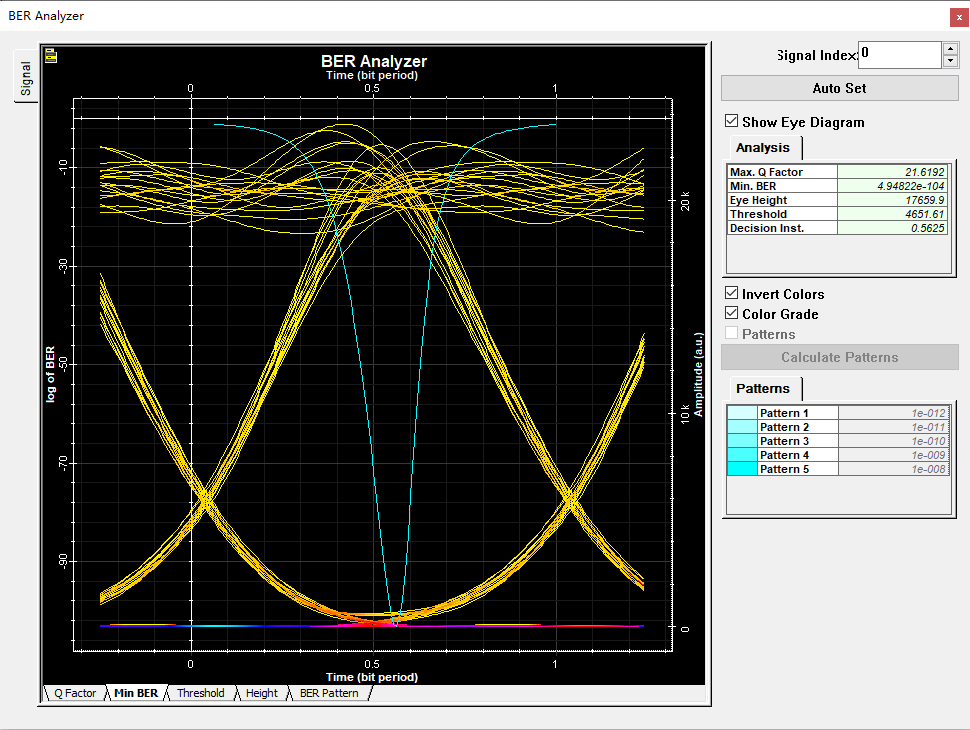
\includegraphics[scale=0.2]{sweep2BER1.png}
        \caption{}
        \label{fig:side:a}
      \end{minipage}%
      \begin{minipage}[t]{0.5\linewidth}
        \centering
        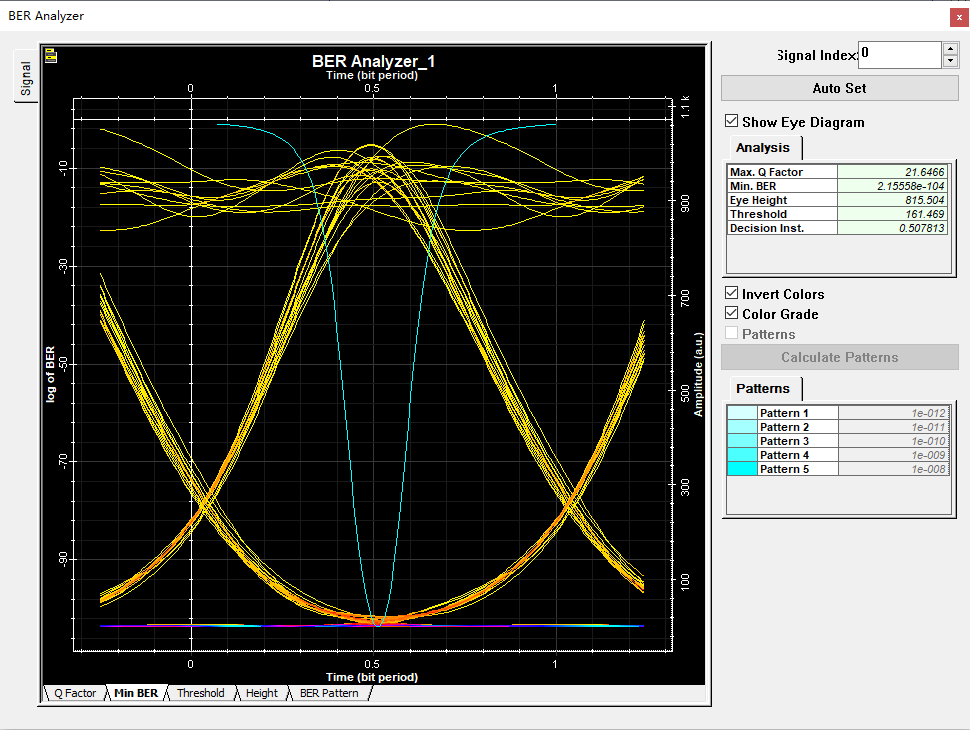
\includegraphics[scale=0.2]{sweep2BER2.png}
        \caption{}
        \label{fig:side:b}
      \end{minipage}
	  \begin{minipage}[t]{0.5\linewidth}
        \centering
        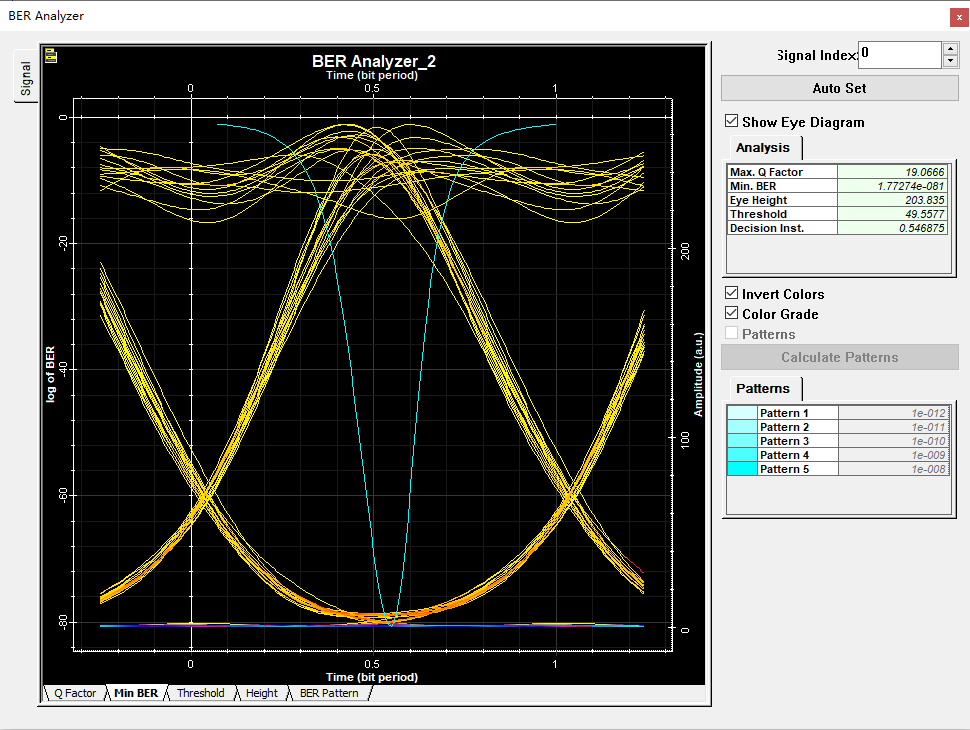
\includegraphics[scale=0.2]{sweep2BER3.png}
        \caption{}
        \label{fig:side:a}
      \end{minipage}%
      \begin{minipage}[t]{0.5\linewidth}
        \centering
        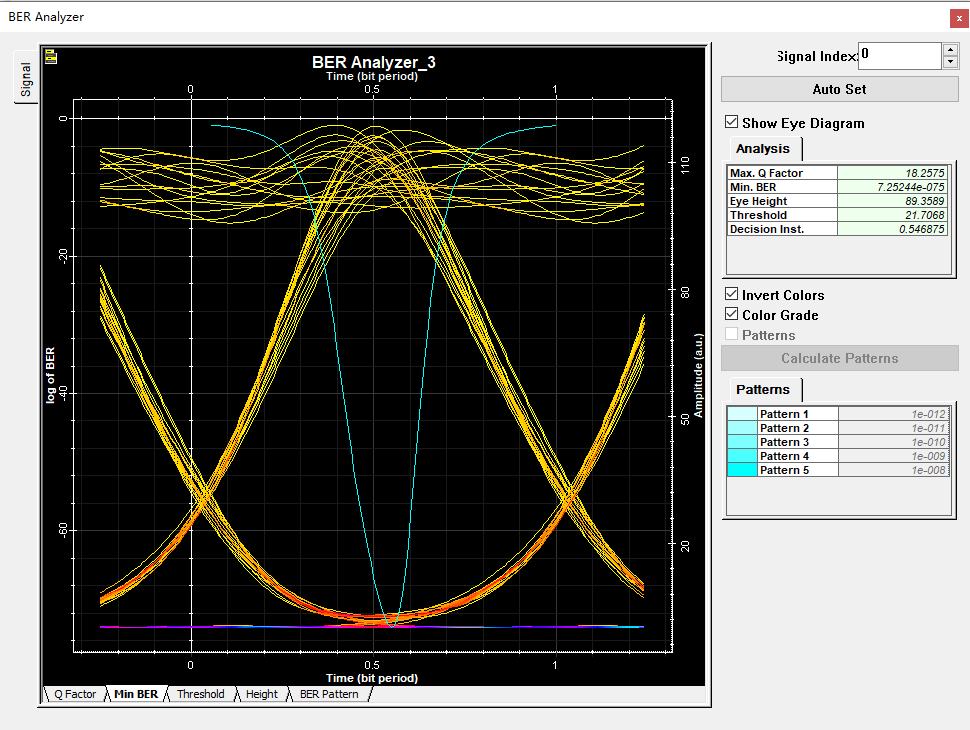
\includegraphics[scale=0.2]{sweep2BER4.png}
        \caption{}
        \label{fig:side:b}
      \end{minipage}
\end{figure}

根据这些图表的分析,我们可以得出结论:随着输入源功率的增加,比特损失率呈现出显著上升的趋势。这表明在高功率输入源下,
光信号的传输质量受到了明显的影响,可能导致数据传输错误率增加。因此,在实际应用中,我们需要仔细控制输入源的功率,
以保持在一个适当的范围内,从而确保信号传输的可靠性和稳定性。

此外,观察到在当前系统下,四个信道的比特损失率相对较低且呈现相似的趋势。这种情况下,即使出现比特损失,可以通过纠错码等技术进行修复,
从而实现对数据的完全恢复。因此,我们可以得出结论,该系统适用于作为四路波分复用信号的传输线路,能够提供可靠的信号传输和较低的比特损失率。

在这个实验中我们可以得出当输入源功率分贝加大时,比特损失率会有非常显著的提升,如下四图所示,
其输入源为0dB其中按顺序分别为193.1THz,193.2THz,193.3THz,193.4THz信号下分析仪得到的眼图以及Q因数和BER(比特损失率)的数据:

\begin{figure}[H]
    \begin{minipage}[t]{0.5\linewidth}
        \centering
        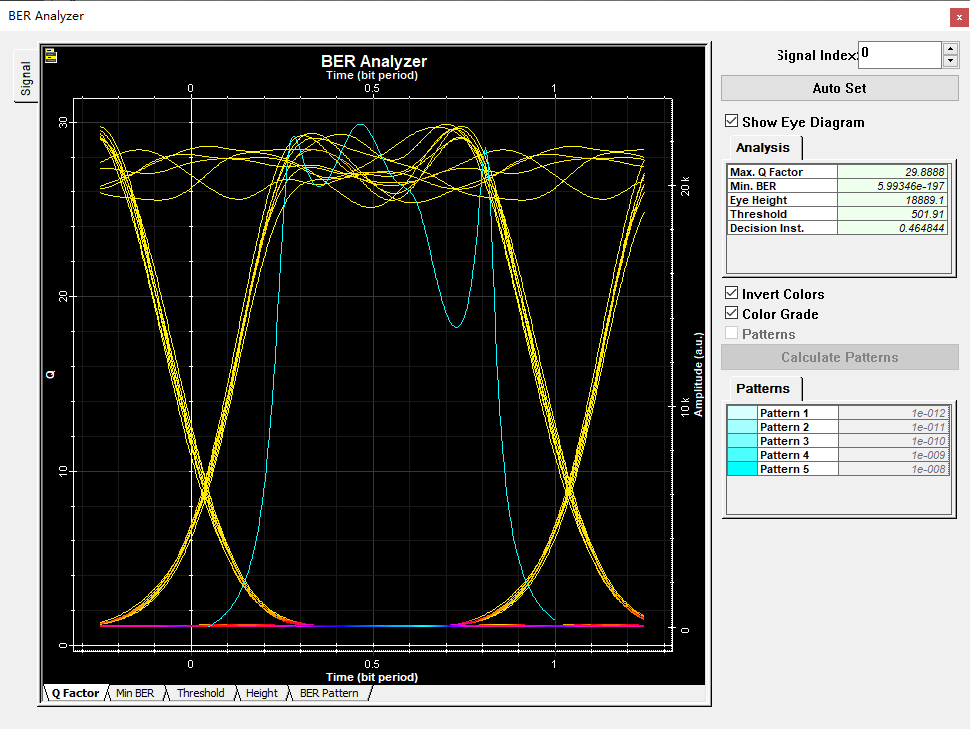
\includegraphics[scale=0.2]{sweep2Q1.png}
        \caption{}
        \label{fig:side:a}
      \end{minipage}%
      \begin{minipage}[t]{0.5\linewidth}
        \centering
        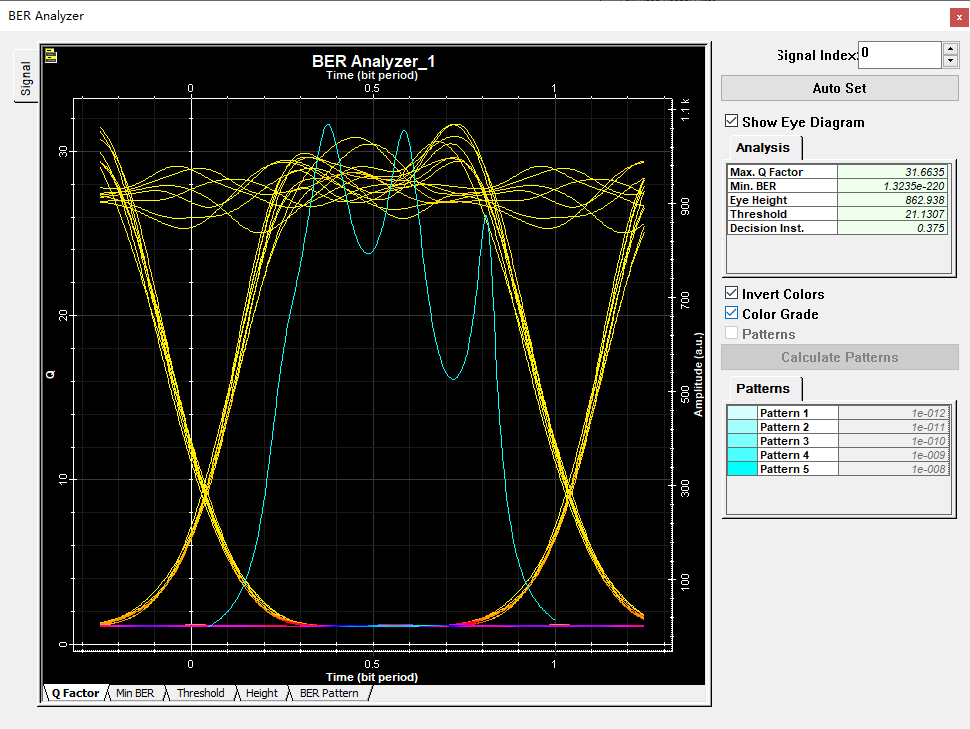
\includegraphics[scale=0.2]{sweep2Q2.png}
        \caption{}
        \label{fig:side:b}
      \end{minipage}
	  \begin{minipage}[t]{0.5\linewidth}
        \centering
        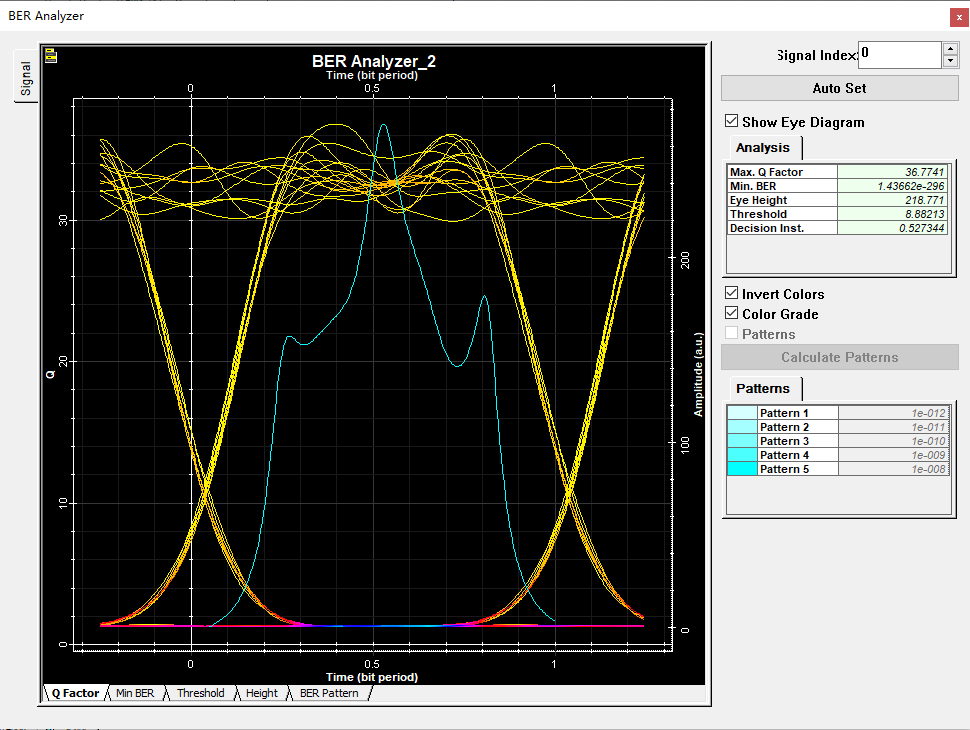
\includegraphics[scale=0.2]{sweep2Q3.png}
        \caption{}
        \label{fig:side:a}
      \end{minipage}%
      \begin{minipage}[t]{0.5\linewidth}
        \centering
        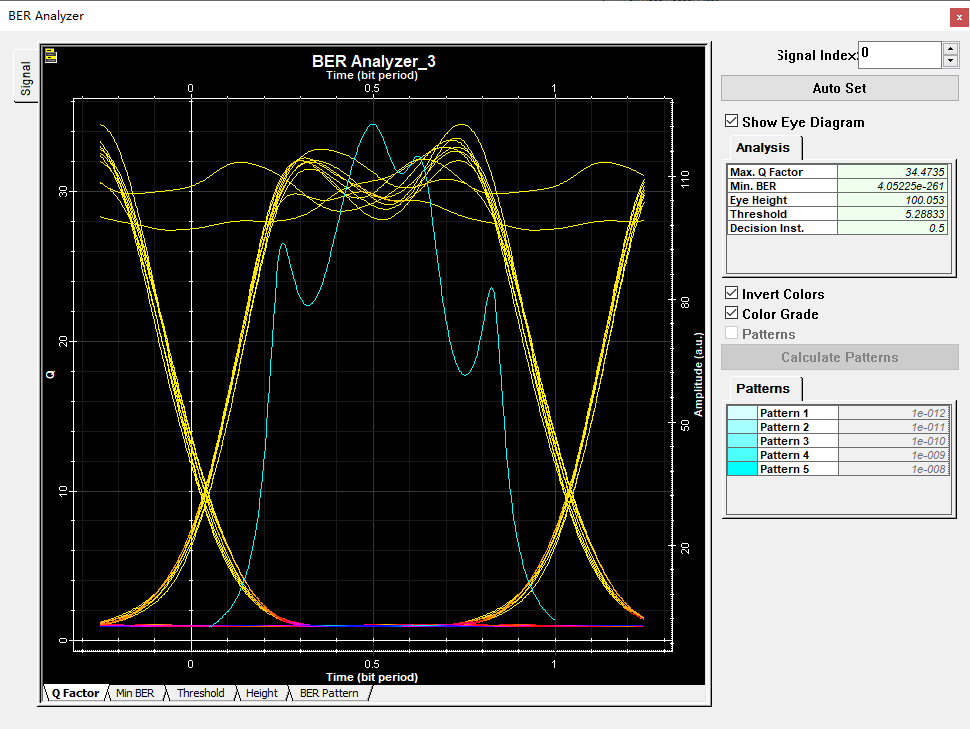
\includegraphics[scale=0.2]{sweep2Q4.png}
        \caption{}
        \label{fig:side:b}
      \end{minipage}
\end{figure}
通过观察图中的结果,我们可以清晰地看到在该情况下比特损失率显著下降。这说明传输精度和输入强度之间存在正相关关系,
即微弱的功耗提升可以大幅改善传输质量。这种性能表现非常符合那些追求高精度信号传输的用户和实验人员的需求。

此外,该系统的Q因子也能够体现出其具有较高质量的信号传输和波分复用失真度极低的特点。Q因子是衡量光纤传输系统性能的重要指标,
其数值越高表示系统的传输质量越好。观察实验数据,我们可以看到在输入源功率增加的情况下,Q因子也随之提高。
这意味着该系统在理论上具有更高的质量,能够应用于更需要精细数据传输的实验和应用环境中。

综上所述,该光纤传输系统展现了显著的性能优势。通过微弱的功耗提升,可以实现比特损失率的大幅下降,从而改善传输质量。
同时,高Q因子的表现说明该系统具有高质量的信号传输和低失真度的波分复用能力。
这些特点使得该系统非常适用于那些对高精度信号传输和精细数据处理要求较高的实验和应用环境,满足了用户和实验人员的需求。

通过上面的说明和比对,我们可以得出结论:在设计中引入色散补偿器和光放大器后,光纤传输系统在Q因子和BER(比特损失率)方面展现出显著的优势。
首先,色散补偿器的应用有效地减小了色散引起的信号畸变和传输损耗。色散是光信号在光纤中传输过程中引起的波形失真现象,
会导致信号的时间展宽和互相重叠,从而降低传输质量。通过使用色散补偿器,我们可以校正和补偿这种失真,
使得信号在传输过程中能够保持较高的质量和准确性。

其次,光放大器的引入提供了信号放大和增益补偿的功能。在长距离传输中,光信号会经历衰减,导致信号强度降低。
通过配置适当的光放大器,我们可以对信号进行放大,使其保持足够的强度和质量。光放大器具有高增益和低噪声的特点,
能够有效地提升信号的传输质量和距离。

综上所述,通过引入色散补偿器和光放大器,我们有效地克服了光纤传输中的色散问题和信号衰减问题。
这使得我们的光纤传输系统在Q因子和BER方面表现出卓越的性能。Q因子是评估信号传输质量的指标,
它与信噪比和误码率相关,而BER则表示单位时间内传输的比特中出现错误的比率。通过优化设计和引入适当的补偿和增益措施,
我们能够实现更高的Q因子和更低的BER,从而提供可靠和高质量的光纤传输。

\clearpage     %另起一页  
\section{总结}
综上所述,我们设计的是一个高性能的光纤传输系统,旨在实现$4\times 5 Gbit/s$的高速数据传输。
通过采用波分复用技术,我们能够将多个不同波长的光信号同时传输在同一根光纤中,从而提高传输容量和利用率。
我们选择了波长间隔为100GHz,并分配了频率为193.1THz、193.2THz、193.3THz和193.4THz的四个通道,每个通道的传输速率为5Gbit/s。

在设计中,我们考虑了光纤损耗和传输距离对信号质量的影响。通过选择常规光纤并控制光纤损耗系数为0.25dB/km,
我们能够保证信号在长达100km的传输距离内仍能保持较低的衰减,从而确保传输质量。此外,我们还要考虑色散对信号的影响。

色散是光信号在光纤中传输过程中的一个关键问题,它会导致不同频率的光信号以不同的速度传播,从而引起信号失真和间隔延迟。
为了解决色散问题,我们引入了色散补偿器。具体地,我们采用了色散补偿光纤(DCF)和光纤光栅(FBG)作为色散补偿器的组成部分。
DCF可以通过负色散来抵消光纤中的色散效应,而FBG则可以通过反射特性来调节不同波长的相位,从而实现色散的补偿。
通过合理配置和优化这些色散补偿器,我们能够有效地减小色散对信号的影响,提高传输质量和系统性能。

此外,我们通过OptiSystem进行了仿真验证,并对系统进行了优化。通过调整系统参数、优化光纤连接和组件配置,
以及采用适当的信号处理策略,我们能够进一步改善系统的传输质量、增强抗干扰能力和降低误码率。

最后,我们的设计方案充分考虑了高速数据传输、波分复用技术的应用、光纤损耗和传输距离的要求,
以及色散补偿器的配置和系统性能优化。通过这些设计措施,我们能够实现高效、可靠的光纤传输,满足现代通信和数据传输的需求。
\clearpage












\pagestyle{headings}
\bibliographystyle{IEEEtran}
\bibliography{qp}

\end{document}
